\chapter{Całki wielokrotne i zamiana zmiennych}
\label{ma2:ch:multiple-integrals}

Przechodzimy od całek na dowolnych zbiorach mierzalnych
do metod ich obliczania przez całki iterowane i zamianę
zmiennych. Ogólne dowody twierdzeń o miarach produktowych
oraz zamianie zmiennych podano odpowiednio w
\atlasref{ME-12::ch:produkty-miary}{ME 12} i
\atlasref{ME-13::ch:zamiana-zmiennych}{ME 13}.
Tutaj rozwijamy rachunek skalarny w przestrzeniach
euklidesowych. Wszystkie miary w tym rozdziale są miarami
Lebesgue'a odpowiednich wymiarów.

\section{Przekroje i całki iterowane}

Niech $m,n\ge1$ będą liczbami naturalnymi.
Dla $E\subseteq\R^m\times\R^n$ określamy przekroje
\[
 E_x=\{y\in\R^n:(x,y)\in E\},\qquad
 E^y=\{x\in\R^m:(x,y)\in E\}.
\]
Jeżeli $f:E\to\R$ jest mierzalna, przedłużamy ją
przez zero poza $E$; analogicznie dla funkcji
nieujemnych o wartościach rozszerzonych.
Takie przedłużenie jest mierzalne, gdy $E$ jest
mierzalny (por. \ref{ma2:prop:lebesgue-zero-extension}).
Dla zbioru Lebesgue'a-mierzalnego nie wszystkie
przekroje muszą być mierzalne. Wynika to z różnicy
pomiędzy produktową $\sigma$-algebrą a jej uzupełnieniem,
omówionej w \atlasref{ME-12::thm:lebesgue-products-12}{ME 12}.

\begin{twierdzenie}[Tonelli w przestrzeni euklidesowej]
\label{ma2:thm:multiple-tonelli}
Jeżeli $f:\R^{m+n}\to[0,\infty]$ jest mierzalna
w sensie Lebesgue'a, to przekroje są mierzalne
dla prawie wszystkich parametrów w odpowiednich
przestrzeniach. Zachodzi
\[
 \begin{aligned}
 \int_{\R^{m+n}} f\,\mathrm d\lambda_{m+n}
 &=\int_{\R^m}\left(\int_{\R^n}f(x,y)\,
   \mathrm d\lambda_n(y)\right)\mathrm d\lambda_m(x)\\
 &=\int_{\R^n}\left(\int_{\R^m}f(x,y)\,
   \mathrm d\lambda_m(x)\right)\mathrm d\lambda_n(y).
 \end{aligned}
\]
Równości obowiązują w $[0,\infty]$; w całkach
zewnętrznych przypisujemy wartość zero na
mierzalnych zbiorach wyjątkowych.
\end{twierdzenie}

\begin{twierdzenie}[Fubini w przestrzeni euklidesowej]
\label{ma2:thm:multiple-fubini}
Niech $f:\R^{m+n}\to\R$ będzie mierzalna i
\[
 \int_{\R^{m+n}}|f|\,\mathrm d\lambda_{m+n}<\infty.
\]
Wówczas przekroje są całkowalne dla prawie
wszystkich parametrów, a obie całki iterowane
z poprzedniego twierdzenia istnieją jako całki
skończone i są równe całce po $\R^{m+n}$.
Funkcje całek przekrojowych są całkowalne
po nadaniu wartości zero na zbiorach wyjątkowych.
\end{twierdzenie}
Obie tezy wynikają bezpośrednio z
\atlasref{ME-12::thm:completed-product-fubini-12}{twierdzenia dla uzupełnionej miary produktowej}
oraz identyfikacji miary produktowej po uzupełnieniu
z $\lambda_{m+n}$. Wersję dla funkcji $|f|$
można zastosować przed sprawdzeniem całkowalności
$f$: skończoność jednej z całek iterowanych
z $|f|$ wystarcza do zastosowania Fubiniego.

\begin{wniosek}[Całkowanie po przekrojach zbioru]
\label{ma2:cor:multiple-sections}
Jeżeli $E\subseteq\R^{m+n}$ jest mierzalny,
to
\[
 \lambda_{m+n}(E)=
 \int_{\R^m}\lambda_n(E_x)\,\mathrm d\lambda_m(x)
 =\int_{\R^n}\lambda_m(E^y)\,\mathrm d\lambda_n(y).
\]
Dla nieujemnej mierzalnej lub całkowalnej funkcji
$f$ na $E$ zachodzi
\[
 \int_E f\,\mathrm d\lambda_{m+n}
 =\int_{\R^m}
 \left(\int_{E_x}f(x,y)\,\mathrm d\lambda_n(y)\right)
 \mathrm d\lambda_m(x),
\]
oraz analogiczny wzór w odwrotnej kolejności.
Przekroje i ich całki rozumiemy prawie wszędzie.
\end{wniosek}
\begin{proof}
Dla miary zbioru stosujemy
\ref{ma2:thm:multiple-tonelli} do $\chi_E$,
a dla funkcji do jej przedłużenia zerem,
stosując odpowiednio Tonellego albo Fubiniego.
\end{proof}

W szczególności na zbiorze
$E=\{(x,y):a\le x\le b,\ \alpha(x)\le y\le\beta(x)\}$,
gdzie $\alpha,\beta$ są ciągłe i $\alpha\le\beta$,
otrzymujemy
\[
 \int_E f\,\mathrm d\lambda_2
 =\int_a^b\left(\int_{\alpha(x)}^{\beta(x)}
 f(x,y)\,\mathrm d\lambda_1(y)\right)
 \mathrm d\lambda_1(x).
\]
Zbiór $E$ jest zwarty, a wzór wynika z jego
przekrojów. W kolejności odwrotnej trzeba
wyznaczyć przekroje poziome; nie zawsze są one
pojedynczymi przedziałami.

\begin{przyklad}[Zmiana kolejności na obszarze płaskim]
\label{ma2:ex:multiple-order}
Niech $E=\{(x,y):0\le x\le1,\ x^2\le y\le x\}$.
Dla $y\in[0,1]$ nierówności $x^2\le y\le x$
są równoważne $y\le x\le\sqrt y$.
W szczególności
\[
 \lambda_2(E)=\int_0^1(x-x^2)\,\mathrm d\lambda_1(x)
 =\int_0^1(\sqrt y-y)\,\mathrm d\lambda_1(y)=\frac16.
\]
Dla funkcji $f(x,y)=e^{y}$ możemy obliczyć całkę
w kolejności $y$, następnie $x$, lecz pojawi się
całka z $e^{x^2}$. Dobór kolejności zależy od
konkretnej funkcji podcałkowej; sama prostota
granic nie przesądza o łatwości rachunku.
Dla $f(x,y)=e^{y^2}$ zmiana kolejności daje
\[
 \int_E e^{y^2}\,\mathrm d\lambda_2
 =\int_0^1(\sqrt y-y)e^{y^2}\,\mathrm d\lambda_1(y).
\]
Natomiast dla $f(x,y)=e^x$ naturalna jest
kolejność z całkowaniem najpierw względem $y$:
\[
 \int_E e^x\,\mathrm d\lambda_2
 =\int_0^1(x-x^2)e^x\,\mathrm d\lambda_1(x)
 =3-e.
\]
Ostatnią równość otrzymujemy przez dwukrotne
całkowanie przez części lub z funkcji pierwotnej
$(-x^2+3x-3)e^x$.
Wszystkie funkcje są tu ciągłe i ograniczone
na zwartym zbiorze.
\end{przyklad}

\begin{figure}[htbp]
\centering
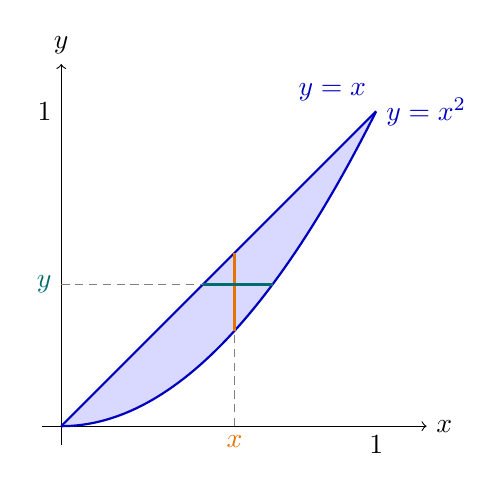
\begin{tikzpicture}[scale=4]
 \fill[blue!15] (0,0)--(1,1)
  plot[domain=1:0,samples=60] (\x,{\x*\x})--cycle;
 \draw[->] (-.06,0)--(1.16,0) node[right] {$x$};
 \draw[->] (0,-.06)--(0,1.15) node[above] {$y$};
 \draw[blue!75!black,thick] (0,0)--(1,1)
  node[above left] {$y=x$};
 \draw[blue!75!black,thick,domain=0:1,samples=60]
  plot (\x,{\x*\x}) node[right] {$y=x^2$};
 \draw[orange!90!black,very thick] (.55,.3025)--(.55,.55);
 \draw[teal!85!black,very thick] (.45,.45)--({sqrt(.45)},.45);
 \node[orange!90!black,below] at (.55,0) {$x$};
 \node[teal!85!black,left] at (0,.45) {$y$};
 \draw[gray,densely dashed] (.55,0)--(.55,.3025);
 \draw[gray,densely dashed] (0,.45)--(.45,.45);
 \node[below] at (1,0) {$1$};
 \node[left] at (0,1) {$1$};
\end{tikzpicture}
\caption{Obszar między parabolą i prostą z przykładu
\ref{ma2:ex:multiple-order}. Pionowy przekrój ma
końce $x^2,x$, a poziomy $y,\sqrt y$.}
\label{ma2:fig:multiple-order}
\end{figure}

\section{Całki iterowane Riemanna i wyjątki}

\begin{stwierdzenie}
\label{ma2:prop:multiple-riemann}
Niech $Q=Q_1\times Q_2$ będzie prostopadłościanem
domkniętym, a $f:Q\to\R$ funkcją całkowalną
w sensie Riemanna. Jeżeli dla każdego $x\in Q_1$
przekrój $f(x,\cdot)$ jest całkowalny w sensie
Riemanna na $Q_2$, to funkcja
\[
 F(x)=\int_{Q_2}f(x,y)\,\mathrm d\lambda_n(y)
\]
jest całkowalna w sensie Riemanna i jej całka
na $Q_1$ jest równa całce $f$ na $Q$.
Wszystkie całki w tej tezie można rozumieć jako
całki Riemanna; zapis Lebesgue'a jest równoważny.
\end{stwierdzenie}
\begin{proof}
Dla podziałów prostokątnych $P_1,P_2$ oznaczmy
przez $m_{ij},M_{ij}$ infimum i supremum $f$
na iloczynie komórek $Q_{1,i}\times Q_{2,j}$.
Dla każdego $x\in Q_{1,i}$ dolna i górna suma
Darboux przekroju dają
\[
 \sum_j m_{ij}\lambda_n(Q_{2,j})
 \le F(x)\le
 \sum_j M_{ij}\lambda_n(Q_{2,j}).
\]
Po pomnożeniu przez objętości $Q_{1,i}$
i zsumowaniu dostajemy
\[
 L(f,P_1\times P_2)\le L(F,P_1)
 \le U(F,P_1)\le U(f,P_1\times P_2).
\]
Każdy podział siatkowy $Q$ jest iloczynem
podziałów siatkowych obu czynników. Z kryterium
Darboux \ref{ma2:thm:riemann-darboux-box}
różnicę zewnętrznych sum można uczynić dowolnie
małą. To samo zachodzi dla $F$, a kresy obu
par sum są równe. Zgodność całek Riemanna
i Lebesgue'a wynika z
\ref{ma2:thm:riemann-box-lebesgue}.
\end{proof}

Jeżeli $f$ jest ciągła na $Q$, wszystkie
przekroje są ciągłe, więc obie kolejności
całkowania są dopuszczalne w sensie Riemanna.
Nie należy jednak utożsamiać tego wyniku
z twierdzeniem Fubiniego dla funkcji mierzalnych,
które dopuszcza zbiory wyjątkowych parametrów.

\begin{przyklad}[Niecałkowalny przekrój Riemanna]
\label{ma2:ex:multiple-riemann-exception}
Na $[0,1]^2$ niech $f(x,y)=\chi_{\{0\}\times(\Q\cap[0,1])}(x,y)$.
Funkcja jest ograniczona, a zbiór jej punktów
nieciągłości jest zawarty w odcinku $\{0\}\times[0,1]$,
który ma zerową miarę $\lambda_2$.
Kryterium Lebesgue'a
\ref{ma2:thm:riemann-box-lebesgue-criterion}
daje całkowalność Riemanna na kwadracie.
Całka wynosi zero, ponieważ funkcja znika
prawie wszędzie. Jednak przekrój $f(0,\cdot)$
jest funkcją Dirichleta, niecałkowalną w sensie
Riemanna. Dla $x>0$ przekroje są identycznie zerowe.
W sensie Lebesgue'a wszystkie przekroje są
całkowalne, a ich całki wynoszą zero.
\end{przyklad}

\begin{przyklad}[Obie całki iterowane istnieją, lecz są różne]
\label{ma2:ex:multiple-nonabsolute}
Na $(0,1)^2$ połóżmy
\[
 f(x,y)=\frac{x^2-y^2}{(x^2+y^2)^2}.
\]
Dla ustalonego $x>0$ mamy
$f(x,y)=\partial_y(y/(x^2+y^2))$, więc
\[
 \int_0^1 f(x,y)\,\mathrm d\lambda_1(y)=\frac1{1+x^2}.
\]
Analogicznie
$f(x,y)=-\partial_x(x/(x^2+y^2))$, skąd
\[
 \int_0^1 f(x,y)\,\mathrm d\lambda_1(x)=-\frac1{1+y^2}.
\]
Całki zewnętrzne dają odpowiednio $\pi/4$ i $-\pi/4$.
Każdy przekrój wewnętrzny jest całkowalny
bezwzględnie, lecz nie zachodzi całkowalność
bezwzględna po całym kwadracie.
Istotnie, na obszarze $0<x<1$, $0<y<x/2$
mamy $x^2-y^2\ge3x^2/4$ oraz
$(x^2+y^2)^2\le25x^4/16$, zatem
$f(x,y)\ge12/(25x^2)$. Tonelli daje
\[
 \int_{(0,1)^2}f^+\,\mathrm d\lambda_2
 \ge\int_0^1\frac{6}{25x}\,\mathrm d\lambda_1(x)=+\infty.
\]
Po zamianie $x,y$ funkcja zmienia znak,
więc analogicznie całka z $f^-$ jest nieskończona.
Całka Lebesgue'a z $f$ po kwadracie nie jest określona.
\end{przyklad}

\section{Więcej niż dwa czynniki}

Dla $d\ge2$ i funkcji nieujemnej mierzalnej na
$\R^d$ albo funkcji całkowalnej stosujemy
\ref{ma2:thm:multiple-tonelli} lub
\ref{ma2:thm:multiple-fubini} kolejno do bloków
współrzędnych. Otrzymujemy dowolną kolejność
$d$ całek jednowymiarowych, z odpowiednimi
wyjątkami prawie wszędzie. Zgodność różnych
grupowań czynników wynika z
\atlasref{ME-12::cor:associative-product-12}{łączności produktu miar}.
Dla iloczynu funkcji nieujemnych $f_i$ na prostej,
gdy wszystkie całki są skończone, dostajemy
\[
 \int_{\R^d}\prod_{i=1}^d f_i(x_i)\,
 \mathrm d\lambda_d(x)=
 \prod_{i=1}^d\int_\R f_i(t)\,\mathrm d\lambda_1(t).
\]
Wynika to z iterowania całek i wyłączania
czynników niezależnych od aktualnej zmiennej.

\begin{przyklad}[Objętość sympleksu]
\label{ma2:ex:multiple-simplex}
Niech $S_d(t)=\{x\in[0,\infty)^d:
\sum_{i=1}^d x_i\le t\}$ dla $t>0$.
Przekroje względem pierwszej współrzędnej
są sympleksami $S_{d-1}(t-u)$ dla $0<u<t$.
Z \ref{ma2:cor:multiple-sections} i indukcji
od $\lambda_1(S_1(t))=t$ otrzymujemy
\[
 \lambda_d(S_d(t))=\int_0^t
 \frac{(t-u)^{d-1}}{(d-1)!}\,\mathrm d\lambda_1(u)
 =\frac{t^d}{d!}.
\]
Ostatnia równość wynika z całkowania potęgi.
\end{przyklad}

\section{Zamiana zmiennych}

\begin{twierdzenie}[Wielowymiarowy wzór na zamianę zmiennych]
\label{ma2:thm:multiple-change}
Niech $U,V\subseteq\R^d$ będą otwarte, a
$\Phi:U\to V$ będzie dyfeomorfizmem klasy $C^1$.
Dla mierzalnego zbioru $E\subseteq U$ zbiór
$\Phi(E)$ jest mierzalny. Jeżeli
$f:\Phi(E)\to[0,\infty]$ jest mierzalna lub
$f:\Phi(E)\to\R$ jest całkowalna, to
\[
 \int_{\Phi(E)} f(y)\,\mathrm d\lambda_d(y)
 =\int_E f(\Phi(x))|\det D\Phi(x)|\,
 \mathrm d\lambda_d(x).
\]
W szczególności
$\lambda_d(\Phi(E))=\int_E|\det D\Phi(x)|
\,\mathrm d\lambda_d(x)$.
\end{twierdzenie}
Dowód ogólny znajduje się w
\atlasref{ME-13::thm:change-variables-13}{ME 13},
a wersja dla podzbiorów w
\atlasref{ME-13::cor:change-subdomain-13}{wniosku o zamianie na podzbiorze}.
Warunki na $\Phi$ można sprawdzić, wykazując
różnowartościowość oraz niezerowość wyznacznika
pochodnej na otwartym zbiorze
(\ref{ma2:cor:inverse-global-injective}).
Wartość bezwzględna wyznacznika jest konieczna,
ponieważ miara objętości jest nieujemna
niezależnie od orientacji.

\begin{przyklad}[Podstawienie afiniczne]
\label{ma2:ex:multiple-affine}
Dla $A\in\mathrm{GL}(d,\R)$ oraz $b\in\R^d$
odwzorowanie $\Phi(x)=Ax+b$ ma pochodną $A$.
Zatem dla dowolnego mierzalnego $E$
\[
 \lambda_d(AE+b)=|\det A|\lambda_d(E).
\]
Jest to też
\atlasref{ME-13::thm:linear-change-13}{liniowy wzór na objętość}.
Jeżeli $a_i>0$ dla $1\le i\le d$, to elipsoida
\[
 E=\left\{y:\sum_{i=1}^d\frac{y_i^2}{a_i^2}<1\right\}
\]
jest obrazem kuli jednostkowej przez macierz
diagonalną z przekątną $(a_1,\ldots,a_d)$.
Jej objętość wynosi $v_d\prod_i a_i$,
gdzie $v_d=\lambda_d(B(0,1))$.
\end{przyklad}

\begin{przyklad}[Podstawienie nieliniowe]
\label{ma2:ex:multiple-nonlinear}
Niech $U=\{(u,v):1<u<2,\ 0<v<1\}$ i
$\Phi(u,v)=(u,uv)$. Na otwartym zbiorze
$\{u>0\}$ odwzorowanie ma gładką odwrotność
$(x,y)\mapsto(x,y/x)$ oraz wyznacznik pochodnej
$u$. Obraz $U$ to
$E=\{(x,y):1<x<2,\ 0<y<x\}$.
Wobec tego
\[
 \int_E \frac{y}{x^2}\,\mathrm d\lambda_2(x,y)
 =\int_U\frac{uv}{u^2}u\,\mathrm d\lambda_2(u,v)
 =\int_1^2\int_0^1 v\,\mathrm d\lambda_1(v)\,
 \mathrm d\lambda_1(u)=\frac12.
\]
W ostatnim kroku stosujemy Fubiniego do
ograniczonej funkcji na ograniczonym zbiorze.
\end{przyklad}

\section{Współrzędne biegunowe, walcowe i sferyczne}

\subsection{Współrzędne biegunowe}

Odwzorowanie
$\Phi(r,\theta)=(r\cos\theta,r\sin\theta)$
dla $r>0$, $0<\theta<2\pi$ jest różnowartościowe,
a jego obraz to płaszczyzna bez nieujemnej półosi
$x_1$. Macierz pochodnej i jej wyznacznik wynoszą
\[
 D\Phi=
 \begin{pmatrix}\cos\theta&-r\sin\theta\\
 \sin\theta&r\cos\theta\end{pmatrix},
 \qquad \det D\Phi=r.
\]
Z niezerowości wyznacznika i
\ref{ma2:cor:inverse-global-injective}
wynika, że jest to dyfeomorfizm na obraz.
Pominięta półoś ma miarę zero, dlatego dla funkcji
nieujemnej mierzalnej lub całkowalnej na $\R^2$
\begin{equation}
 \label{ma2:eq:multiple-polar}
 \int_{\R^2}f\,\mathrm d\lambda_2
 =\int_0^{2\pi}\int_0^\infty
 f(r\cos\theta,r\sin\theta)r\,
 \mathrm d\lambda_1(r)\,\mathrm d\lambda_1(\theta).
\end{equation}
Stosujemy \ref{ma2:thm:multiple-change}
oraz Tonellego albo Fubiniego.
Dla całki na podzbiorze należy przedłużyć
funkcję przez zero lub ograniczyć dziedzinę
parametrów do odpowiedniego przeciwobrazu.

\begin{przyklad}[Całka Gaussa]
\label{ma2:ex:multiple-gaussian}
Oznaczmy $I=\int_\R e^{-t^2}\,\mathrm d\lambda_1(t)$.
Jest to całka dodatnia i skończona, ponieważ
dla $|t|\ge1$ mamy $e^{-t^2}\le e^{-|t|}$.
Z Tonellego i \ref{ma2:eq:multiple-polar}
wynika
\[
 I^2=\int_{\R^2}e^{-(x_1^2+x_2^2)}\,\mathrm d\lambda_2(x)
 =2\pi\int_0^\infty e^{-r^2}r\,\mathrm d\lambda_1(r)=\pi.
\]
Podstawienie $u=r^2$ daje ostatnią równość.
Zatem $I=\sqrt\pi$.
\end{przyklad}

\subsection{Współrzędne walcowe}

Odwzorowanie
\[
 \Psi(r,\theta,z)=(r\cos\theta,r\sin\theta,z)
\]
na $(0,\infty)\times(0,2\pi)\times\R$
jest iloczynem odwzorowania biegunowego
i tożsamości. Jest dyfeomorfizmem na
$\R^3\setminus\{(x_1,0,x_3):x_1\ge0\}$,
a jego wyznacznik pochodnej wynosi $r$,
ponieważ macierz jest blokowo diagonalna.
Pominięty zbiór leży w płaszczyźnie, więc ma
miarę $\lambda_3$ zero. Stąd
\[
 \int_{\R^3} f\,\mathrm d\lambda_3
 =\int_\R\int_0^{2\pi}\int_0^\infty
 f(r\cos\theta,r\sin\theta,z)\,r\,
 \mathrm d\lambda_1(r)\,\mathrm d\lambda_1(\theta)\,
 \mathrm d\lambda_1(z)
\]
dla funkcji nieujemnych mierzalnych lub całkowalnych,
na mocy \ref{ma2:thm:multiple-change}
i twierdzeń o całkach iterowanych.

\begin{przyklad}[Bryła pod paraboloidą]
\label{ma2:ex:multiple-paraboloid}
Niech $R>0$ oraz
$E=\{(x_1,x_2,z):0\le z\le R^2-x_1^2-x_2^2\}$.
We współrzędnych walcowych otrzymujemy
$0\le r\le R$, $0\le z\le R^2-r^2$,
$0<\theta<2\pi$, z pominięciem zbioru miary zero.
Zatem
\[
 \lambda_3(E)=2\pi\int_0^R r(R^2-r^2)\,
 \mathrm d\lambda_1(r)=\frac{\pi R^4}{2}.
\]
Równość wynika z całkowania wielomianu.
\end{przyklad}

\subsection{Współrzędne sferyczne}

Ustalamy konwencję: $\rho$ to odległość od zera,
$\varphi$ to kąt od dodatniej półosi $x_3$,
a $\theta$ to azymut. Dla
$\rho>0$, $0<\varphi<\pi$, $0<\theta<2\pi$
określamy
\[
 \Xi(\rho,\varphi,\theta)=
 (\rho\sin\varphi\cos\theta,\,
 \rho\sin\varphi\sin\theta,\,
 \rho\cos\varphi).
\]
Obraz jest dopełnieniem półpłaszczyzny
$\{(x_1,0,x_3):x_1\ge0\}$. Istotnie, poza nią
$\rho=\|x\|_2>0$, kąt
$\varphi=\arccos(x_3/\rho)$ należy do $(0,\pi)$,
a azymut jest jednoznacznie określony jak dla
współrzędnych biegunowych. To dowodzi
różnowartościowości i opisu obrazu.
Kolumny macierzy pochodnej wynoszą
\[
 \begin{pmatrix}
 \sin\varphi\cos\theta\\ \sin\varphi\sin\theta\\ \cos\varphi
 \end{pmatrix},\quad
 \rho\begin{pmatrix}
 \cos\varphi\cos\theta\\ \cos\varphi\sin\theta\\-\sin\varphi
 \end{pmatrix},\quad
 \rho\sin\varphi\begin{pmatrix}-\sin\theta\\\cos\theta\\0
 \end{pmatrix}.
\]
Po wyłączeniu czynników $\rho$ i $\rho\sin\varphi$
pozostają trzy wektory ortonormalne: ich normy
są równe $1$, a iloczyny skalarne zero
na mocy tożsamości trygonometrycznych.
Wobec tego
$|\det D\Xi|=\rho^2\sin\varphi>0$.
Z \ref{ma2:cor:inverse-global-injective}
wynika własność dyfeomorfizmu.
Pominięta półpłaszczyzna ma miarę zero.
Otrzymujemy więc
\begin{equation}
\label{ma2:eq:multiple-spherical}
 \begin{split}
 \int_{\R^3} f\,\mathrm d\lambda_3
 ={}&\int_0^{2\pi}\int_0^\pi\int_0^\infty
 f(\Xi(\rho,\varphi,\theta))\rho^2\sin\varphi\\
 &\quad\mathrm d\lambda_1(\rho)\,
 \mathrm d\lambda_1(\varphi)\,
 \mathrm d\lambda_1(\theta)
 \end{split}
\end{equation}
dla funkcji nieujemnych mierzalnych lub całkowalnych.
Podobnie jak we współrzędnych biegunowych,
całki na podzbiorach obliczamy przez
odpowiednie ograniczenie parametrów.

\begin{przyklad}[Objętość kuli i moment radialny]
\label{ma2:ex:multiple-ball-volume}
Dla $R>0$ ze wzoru \ref{ma2:eq:multiple-spherical}
stosowanego do funkcji charakterystycznej kuli
otrzymujemy
\[
 \lambda_3(B(0,R))=
 2\pi\left(\int_0^\pi\sin\varphi\,\mathrm d\lambda_1(\varphi)\right)
 \left(\int_0^R\rho^2\,\mathrm d\lambda_1(\rho)\right)
 =\frac{4\pi R^3}{3}.
\]
W szczególności $v_3=4\pi/3$. Dla $p>-3$
ten sam rachunek z czynnikiem $\rho^p$ daje
\[
 \int_{B(0,R)\setminus\{0\}}\|x\|_2^p\,
 \mathrm d\lambda_3(x)=\frac{4\pi R^{p+3}}{p+3}.
\]
Jest to zgodne ze wzorem radialnym
\ref{ma2:thm:improper-radial}, wyprowadzonym
wcześniej bez współrzędnych biegunowych.
\end{przyklad}

W zamianie zmiennych należy zawsze sprawdzić
dziedzinę parametrów, różnowartościowość,
wyznacznik pochodnej i miarę pominiętych zbiorów.
Przedłużenie zakresu kąta azymutalnego ponad
pełny obrót prowadzi do wielokrotnego pokrycia
obrazu; nie wolno wówczas bezpośrednio stosować
wzoru dla dyfeomorfizmu. W rachunku całek
krzywoliniowych i powierzchniowych analogiczną
rolę będzie odgrywać macierz Grama, a przy
nieróżnowartościowych parametryzacjach krotność.
